% ============================================================================
% Technical Report: Pineapple-Bot-Pro
% Vietnam Robotics For Good — National Competition
% Hosted at USTH (Dai Hoc Viet Phap)
% ============================================================================

\documentclass[12pt, a4paper, twoside]{article}

% --- Packages ---
\usepackage[utf8]{inputenc}
\usepackage[T5,T1]{fontenc}
\usepackage{lmodern}
\usepackage[english]{babel}
\usepackage{geometry}
\geometry{
    a4paper,
    top=25mm,
    bottom=25mm,
    left=25mm,
    right=25mm,
    headheight=14.5pt
}
\usepackage{amsmath, amssymb, amsfonts}
\usepackage{graphicx}
\usepackage{booktabs}
\usepackage{tabularx}
\usepackage{multirow}
\usepackage{enumitem}
\usepackage{float}
\usepackage{caption}
\usepackage{subcaption}
\usepackage{csquotes} % Added to fix biblatex warning
\usepackage{hyperref}
\hypersetup{
    colorlinks=true,
    linkcolor=blue!70!black,
    citecolor=green!50!black,
    urlcolor=blue!60!black,
    pdftitle={Pineapple-Bot-Pro: Technical Report},
    pdfauthor={Team Pineapple}
}
\usepackage{listings}
\usepackage{xcolor}
\usepackage{tikz}
\usetikzlibrary{arrows.meta, positioning, shapes.geometric, fit, calc, decorations.pathreplacing}
\usepackage{pgfplots}
\pgfplotsset{compat=1.18}
\usepackage{fancyhdr}
\usepackage{titlesec}
\usepackage{algorithm}
\usepackage{algpseudocode}
\usepackage[backend=biber, style=ieee]{biblatex}
\usepackage{siunitx}
\usepackage{cleveref}

% --- Header / Footer ---
\pagestyle{fancy}
\fancyhf{}
\fancyhead[LE,RO]{\thepage}
\fancyhead[LO]{\nouppercase{\leftmark}}
\fancyhead[RE]{Pineapple-Bot-Pro: Technical Report}
\renewcommand{\headrulewidth}{0.4pt}

% --- Code Listing Style ---
\lstdefinestyle{cppstyle}{
    language=C++,
    basicstyle=\ttfamily\footnotesize,
    keywordstyle=\color{blue!80!black}\bfseries,
    commentstyle=\color{green!50!black}\itshape,
    stringstyle=\color{red!70!black},
    numbers=left,
    numberstyle=\tiny\color{gray},
    numbersep=5pt,
    frame=single,
    breaklines=true,
    captionpos=b,
    tabsize=4
}

\lstdefinestyle{kotlinstyle}{
    language=Java,
    basicstyle=\ttfamily\footnotesize,
    keywordstyle=\color{blue!80!black}\bfseries,
    commentstyle=\color{green!50!black}\itshape,
    stringstyle=\color{red!70!black},
    numbers=left,
    numberstyle=\tiny\color{gray},
    numbersep=5pt,
    frame=single,
    breaklines=true,
    captionpos=b,
    tabsize=4,
    morekeywords={val, var, fun, data, class, object, when, companion, override, suspend, private, internal, sealed, enum}
}

% --- Section Formatting ---
\titleformat{\section}{\Large\bfseries}{\thesection}{1em}{}
\titleformat{\subsection}{\large\bfseries}{\thesubsection}{1em}{}
\titleformat{\subsubsection}{\normalsize\bfseries}{\thesubsubsection}{1em}{}

% --- Custom Commands ---
\newcommand{\unitmm}{\,\text{mm}}
\newcommand{\unitms}{\,\text{ms}}
\newcommand{\unitHz}{\,\text{Hz}}
\newcommand{\unitkHz}{\,\text{kHz}}
\newcommand{\unitmms}{\,\text{mm/s}}
\newcommand{\unitmmss}{\,\text{mm/s}^2}
\newcommand{\unitmmsss}{\,\text{mm/s}^3}
\newcommand{\unitdegs}{\,\text{deg/s}}
\newcommand{\unitdegss}{\,\text{deg/s}^2}

% ============================================================================
\begin{document}

% --- Title Page ---
\begin{titlepage}
    \centering
    \vspace*{2cm}

    {\Huge\bfseries Pineapple-Bot-Pro}\\[0.5cm]
    {\LARGE\itshape A Low-Cost Mecanum-Drive Robot with\\Latency-Compensated Vision and\\Jerk-Limited Trajectory Control}\\[2cm]

    {\Large\bfseries Technical Report}\\[0.5cm]
    {\large Vietnam Robotics For Good --- National Competition}\\[0.3cm]
    {\large Hosted at USTH ({\fontencoding{T5}\selectfont Đại Học Việt Pháp})}\\[2.5cm]

    {\Large Team Pineapple}\\[2cm]

    \vfill

    {\large April 2026}
\end{titlepage}

% --- Table of Contents ---
\newpage
\tableofcontents
\newpage

% ============================================================================
\section{Abstract}
% ============================================================================

This report presents the design and implementation of the \textbf{Pineapple-Bot-Pro}, an autonomous mecanum-wheeled robot system developed for the \emph{Vietnam Robotics For Good} national competition. The system is built on a deliberately constrained, low-cost hardware platform centered on an ESP32-S3 microcontroller, commodity brushed motors, and Tower Pro SG90 micro-servos, demonstrating that sophisticated autonomous behavior can be achieved without expensive sensors or actuators.

The primary contribution of this work is a tightly integrated software architecture spanning two distinct platforms---an ESP32-S3 embedded firmware and an Android companion application---that together implement several novel techniques for overcoming the limitations of low-cost hardware. These include: (1)~an \emph{asymmetric dual-core firmware architecture} that dedicates one processor core to a \SI{1}{\kilo\hertz} motor control loop while the other handles network communication; (2)~a \emph{jerk-limited S-curve trajectory profiler} with velocity and acceleration feedforward compensation; (3)~a \emph{latency-compensated vision system} that uses historical dead-reckoning state to retroactively correct for the {$\sim$\SI{150}{\milli\second}} camera-to-actuation delay inherent in smartphone-based tracking; (4)~a \emph{single-motor micro-adjustment mode} that exploits mecanum kinematics to achieve sub-\SI{2}{\milli\metre} positional corrections; and (5)~a \emph{physics-based predictive braking system} with an adaptive lookahead that scales with robot velocity.

The system achieves reliable waypoint navigation with $\pm$\SI{5}{\milli\metre} positional tolerance and $\pm 1.5^\circ$ angular tolerance on a \SI{1143}{\milli\metre} $\times$ \SI{1181}{\milli\metre} competition field, using only a consumer smartphone camera for external localization.

% ============================================================================
\section{Introduction}
\label{sec:introduction}
% ============================================================================

\subsection{Competition Context}

The \emph{Vietnam Robotics For Good} competition challenges teams to design autonomous robotic systems capable of performing precision manipulation tasks on a structured playing field. The competition emphasizes practical engineering under real-world constraints: limited budgets, unreliable network conditions, and the demand for robust autonomous operation without human intervention during runs.

The Pineapple-Bot-Pro system was developed under a deliberate philosophy of \emph{cost-constrained sophistication}. Rather than investing in high-end hardware---industrial servo motors, LiDAR sensors, or dedicated vision processors---the team elected to maximize the algorithmic and architectural complexity of the software stack running on commodity components. This approach demonstrates that careful systems engineering can compensate for hardware limitations, a principle with broad applicability beyond competitive robotics.

\subsection{System Overview}

The Pineapple-Bot-Pro system comprises two tightly coupled subsystems:

\begin{enumerate}[label=\arabic*.]
    \item \textbf{Robot Firmware}: A PlatformIO-based C++ application running on an ESP32-S3 microcontroller. The firmware implements a dual-core architecture with dedicated tasks for motor control (\SI{1}{\kilo\hertz} on Core~1) and network communication (Core~0). Key subsystems include a 16-segment motion queue with S-curve trajectory profiling, a Kalman-filtered dead-reckoning engine with camera-based latency compensation, and a four-motor mecanum drive controller with multiple operating modes.

    \item \textbf{Android Controller Application}: A Kotlin/Jetpack Compose application that serves as both the external vision system and the mission sequencer. The app uses the smartphone's rear camera with OpenCV-based ArUco marker detection to provide real-time position and orientation observations of the robot on the playing field. It implements a graph-based path editor, a continuous motion controller with waypoint sequencing, and a structured UDP communication bridge for robot telemetry and command dispatch.
\end{enumerate}

\Cref{fig:system-overview} illustrates the high-level architecture.

\begin{figure}[H]
    \centering
    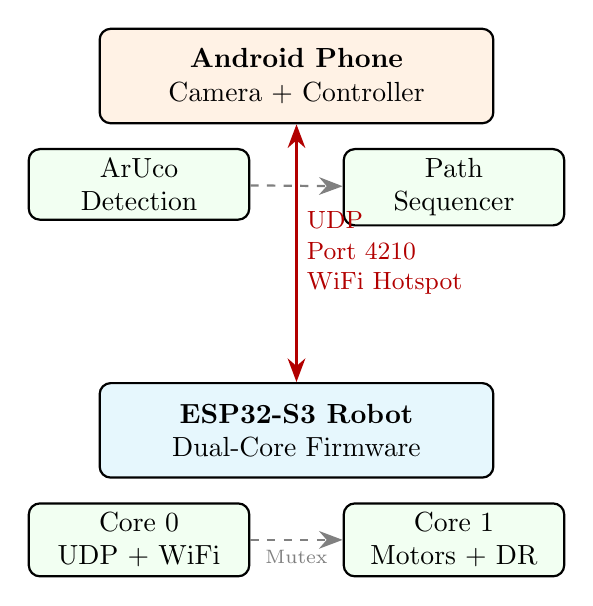
\begin{tikzpicture}[
        block/.style={rectangle, draw, rounded corners, minimum height=1.2cm, minimum width=3.5cm, align=center, thick, fill=blue!5},
        smallblock/.style={rectangle, draw, rounded corners, minimum height=0.8cm, minimum width=2.8cm, align=center, thick, fill=green!5},
        arrow/.style={-{Stealth[length=3mm]}, thick},
        doublearrow/.style={{Stealth[length=3mm]}-{Stealth[length=3mm]}, thick}
    ]
        % Phone
        \node[block, fill=orange!10, minimum width=5cm] (phone) at (0,0) {\textbf{Android Phone}\\Camera + Controller};
        \node[smallblock, below=0.3cm of phone, xshift=-2cm] (cam) {ArUco\\Detection};
        \node[smallblock, below=0.3cm of phone, xshift=2cm] (seq) {Path\\Sequencer};

        % Robot
        \node[block, fill=cyan!10, minimum width=5cm] (robot) at (0,-4.5) {\textbf{ESP32-S3 Robot}\\Dual-Core Firmware};
        \node[smallblock, below=0.3cm of robot, xshift=-2cm] (core0) {Core 0\\UDP + WiFi};
        \node[smallblock, below=0.3cm of robot, xshift=2cm] (core1) {Core 1\\Motors + DR};

        % UDP link
        \draw[doublearrow, red!70!black] (phone.south) -- node[right, align=left, font=\small] {UDP\\Port 4210\\WiFi Hotspot} (robot.north);

        % Internal connections
        \draw[arrow, dashed, gray] (cam) -- (seq);
        \draw[arrow, dashed, gray] (core0) -- (core1) node[midway, below, font=\scriptsize] {Mutex};
    \end{tikzpicture}
    \caption{High-level system architecture. The Android phone acts as both the external vision sensor and the mission controller, communicating with the robot over a direct WiFi hotspot link via UDP on port~4210.}
    \label{fig:system-overview}
\end{figure}

\subsection{Design Philosophy}

Several guiding principles shaped the system design:

\begin{itemize}
    \item \textbf{Software Over Hardware:} Invest in algorithmic sophistication rather than expensive components. A \$3 ESP32-S3 can execute a \SI{1}{\kilo\hertz} control loop with S-curve profiling, Kalman filtering, and predictive braking---capabilities typically associated with dedicated motion controllers costing orders of magnitude more.

    \item \textbf{Graceful Degradation:} The system must remain functional even when individual subsystems fail. If camera observations stop arriving, the robot continues on dead reckoning. If network latency spikes, the latency-aware speed governor prevents overshoot.

    \item \textbf{Multi-Robot Generality:} The firmware supports a layered configuration system that allows the same codebase to run on physically distinct robots with different calibration parameters, mass distributions, and servo configurations.
\end{itemize}

% ============================================================================
\section{Hardware Platform}
\label{sec:hardware}
% ============================================================================

\subsection{Microcontroller}

The robot is powered by the \textbf{Espressif ESP32-S3-DevKitM-1}, a dual-core Xtensa LX7 processor clocked at \SI{240}{\mega\hertz}. The ESP32-S3 was selected for its combination of dual-core processing capability, integrated WiFi (802.11 b/g/n), generous SRAM (\SI{512}{\kilo\byte}), and extremely low unit cost (\textasciitilde\$3 USD). The Arduino framework is used via PlatformIO for development convenience, with FreeRTOS primitives (mutexes, task pinning) employed for explicit dual-core scheduling.

Key configuration parameters from \texttt{platformio.ini}:
\begin{itemize}
    \item CPU frequency: \SI{240}{\mega\hertz}
    \item Framework: Arduino (ESP-IDF underneath)
    \item Serial monitor: \SI{921600}{baud}
    \item USB mode: CDC-on-boot for seamless serial debugging
\end{itemize}

\subsection{Drive System}

The robot employs a \textbf{four-wheel mecanum drive} using brushed DC motors (speculative model: ST130-12240-38 or equivalent). Mecanum wheels were chosen for their holonomic mobility---the ability to translate in any direction without rotating the chassis---which is essential for the precision positioning tasks required by the competition.

The motors are driven via a PWM-based H-bridge controller library (\texttt{ESP32\_Motor\_Controller}), with duty cycles ranging from 0 to 100. The wheel layout follows a standard mecanum configuration:

\begin{table}[H]
    \centering
    \caption{Motor assignment and layout.}
    \label{tab:motor-layout}
    \begin{tabular}{@{}llll@{}}
        \toprule
        \textbf{Motor} & \textbf{Position} & \textbf{Side} & \textbf{Balance Offset} \\
        \midrule
        M1 & Front Right  & Right & $-3.0$ duty \\
        M2 & Front Left   & Left  & --- \\
        M3 & Back Left    & Left  & --- \\
        M4 & Back Right   & Right & $-3.0$ duty \\
        \bottomrule
    \end{tabular}
\end{table}

\noindent Motors M1 and M2 are configured with reversed polarity in firmware to account for opposite physical mounting orientations.

\subsection{Servo Actuators}

The robot uses up to four \textbf{Tower Pro SG90} micro-servos for manipulation tasks. The SG90 is an ultra-low-cost (\textasciitilde\$1 USD) hobby servo with the following nominal specifications:

\begin{table}[H]
    \centering
    \caption{Tower Pro SG90 servo specifications (nominal).}
    \label{tab:sg90-specs}
    \begin{tabular}{@{}ll@{}}
        \toprule
        \textbf{Parameter} & \textbf{Value} \\
        \midrule
        Operating voltage & \SIrange{4.8}{6.0}{\volt} \\
        Stall torque      & \SI{1.8}{\kilogram\cdot\centi\metre} at \SI{4.8}{\volt} \\
        Operating speed   & \SI{0.1}{\second} / \SI{60}{\degree} \\
        Rotation range    & \SI{180}{\degree} \\
        Weight            & \SI{9}{\gram} \\
        \bottomrule
    \end{tabular}
\end{table}

The firmware supports two distinct servo configurations, conditionally compiled for each robot:

\begin{itemize}
    \item \textbf{Robot~A (Fruit Picker):} Three servos configured as a grabber (left/right/center sweep), a vertical slider (up/down), and an arm (up/down). Combined, these enable compound pick-and-place sequences such as \texttt{LOWER\_LEFT}, \texttt{UPPER\_RIGHT}, etc.

    \item \textbf{Robot~B (Dispenser):} Two servos configured as a dropper (open/close) and a ceiling mechanism (open/close/water).
\end{itemize}

\subsection{Communication Hardware}

Rather than employing a dedicated radio link (e.g., Bluetooth, LoRa, or XBee), the system uses the ESP32-S3's \textbf{integrated WiFi} to connect to an Android phone configured as a mobile hotspot. This eliminates the need for additional transceiver hardware and leverages the smartphone's existing networking stack. The phone's gateway IP is automatically used as the command endpoint, requiring zero manual network configuration.

\subsection{External Vision System}

The external localization system is the \textbf{smartphone's rear camera}, processed via CameraX with OpenCV. This deliberately eschews dedicated vision hardware (e.g., Intel RealSense, overhead cameras with dedicated PCs) in favour of a single consumer device that also serves as the mission controller, minimizing both cost and physical setup complexity.

\subsection{Physical Specifications}

Two robot configurations are supported, with the key physical parameters summarized in \Cref{tab:physical-specs}.

\begin{table}[H]
    \centering
    \caption{Physical specifications of Robot~A and Robot~B.}
    \label{tab:physical-specs}
    \begin{tabular}{@{}lll@{}}
        \toprule
        \textbf{Parameter} & \textbf{Robot A} & \textbf{Robot B} \\
        \midrule
        Mass                          & \SI{460}{\gram}   & \SI{926.3}{\gram}   \\
        Actuation force (vertical)     & \SI{3.79}{\newton} & Variable \\
        Static friction coefficient    & 0.847              & 0.372 \\
        Traction limit                 & \SI{8308}{mm/s^2}  & \SI{3652}{mm/s^2} \\
        Motor torque limit             & \SI{8242}{mm/s^2}  & --- \\
        Dominant constraint            & Motor-limited      & Traction-limited \\
        \bottomrule
    \end{tabular}
\end{table}

The kinematic implications of these measurements are significant: Robot~A is \emph{traction-dominant}---the motors physically cannot output enough torque to break traction, making it inherently immune to acceleration-induced slip. Robot~B, conversely, is \emph{traction-limited}, requiring firmware-enforced acceleration caps to prevent wheel slip and ensure dead-reckoning accuracy.

% ============================================================================
\section{Firmware Architecture}
\label{sec:firmware}
% ============================================================================

\subsection{Asymmetric Dual-Core Design}

The ESP32-S3's dual Xtensa LX7 cores are partitioned asymmetrically:

\begin{itemize}
    \item \textbf{Core~0 (Network \& Parsing):} Runs the \texttt{udpTask} as a FreeRTOS task at priority~2. This core handles WiFi stack events, asynchronous UDP packet reception and parsing, and periodic telemetry broadcasting (STATUS at \SI{10}{\hertz}, HELLO at \SI{0.33}{\hertz}, PING at \SI{2}{\hertz}).

    \item \textbf{Core~1 (Motion \& Kinematics):} Runs the Arduino \texttt{loop()} function, dedicated to the high-frequency motor control loop targeting \textbf{\SI{1}{\kilo\hertz}} (\SI{1}{\milli\second} interval). This core processes the motion queue, computes trajectory profiles, updates dead reckoning, and drives the motors.
\end{itemize}

State synchronization between cores is managed via a single FreeRTOS mutex (\texttt{stateMutex}) that guards access to the shared motion queue, dead reckoning engine, and latency compensator. The ABORT command is given special priority: Core~0 sets a volatile \texttt{abortFlag} that Core~1 checks at the top of every control loop iteration, enabling sub-millisecond emergency stop response without waiting for the mutex.

\begin{figure}[H]
    \centering
    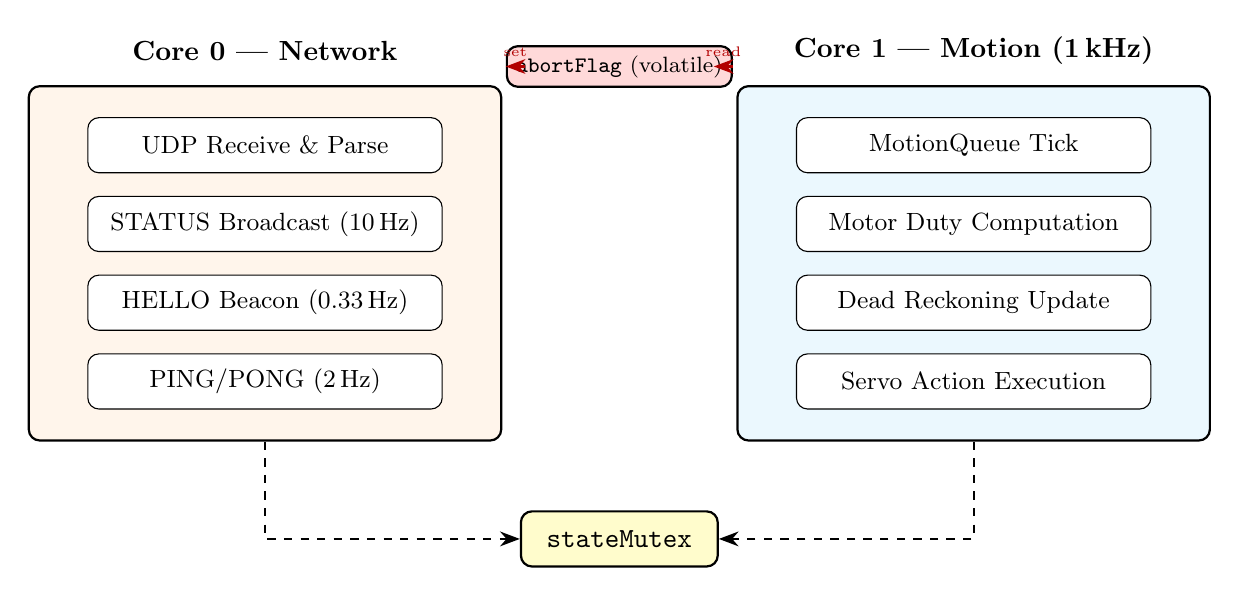
\begin{tikzpicture}[
        core/.style={rectangle, draw, thick, rounded corners, minimum width=6cm, minimum height=4.5cm, fill=#1},
        task/.style={rectangle, draw, rounded corners, minimum height=0.7cm, minimum width=4.5cm, align=center, font=\small, fill=white},
        arrow/.style={-{Stealth[length=2.5mm]}, thick},
        brace/.style={decorate, decoration={brace, amplitude=8pt, raise=4pt}}
    ]
        % Core 0
        \node[core=orange!8] (c0) at (-4.5,0) {};
        \node[font=\bfseries] at (-4.5, 2.7) {Core 0 --- Network};
        \node[task] (udp) at (-4.5, 1.5) {UDP Receive \& Parse};
        \node[task] (status) at (-4.5, 0.5) {STATUS Broadcast (10\,Hz)};
        \node[task] (hello) at (-4.5, -0.5) {HELLO Beacon (0.33\,Hz)};
        \node[task] (ping) at (-4.5, -1.5) {PING/PONG (2\,Hz)};

        % Core 1
        \node[core=cyan!8] (c1) at (4.5,0) {};
        \node[font=\bfseries] at (4.5, 2.7) {Core 1 --- Motion (1\,kHz)};
        \node[task] (mq) at (4.5, 1.5) {MotionQueue Tick};
        \node[task] (motors) at (4.5, 0.5) {Motor Duty Computation};
        \node[task] (dr) at (4.5, -0.5) {Dead Reckoning Update};
        \node[task] (servo) at (4.5, -1.5) {Servo Action Execution};

        % Mutex
        \node[draw, thick, fill=yellow!20, rounded corners, minimum height=0.7cm, minimum width=2.5cm, align=center] (mutex) at (0, -3.5) {\texttt{stateMutex}};
        \draw[arrow, dashed] (c0.south) |- (mutex.west);
        \draw[arrow, dashed] (c1.south) |- (mutex.east);

        % Abort flag
        \node[draw, thick, fill=red!15, rounded corners, minimum height=0.5cm, font=\footnotesize] (abort) at (0, 2.5) {\texttt{abortFlag} (volatile)};
        \draw[arrow, red!70!black] (-1.2, 2.5) -- (abort.west) node[midway, above, font=\tiny] {set};
        \draw[arrow, red!70!black] (abort.east) -- (1.2, 2.5) node[midway, above, font=\tiny] {read};
    \end{tikzpicture}
    \caption{Dual-core task partitioning. Core~0 handles all network I/O while Core~1 runs the deterministic \SI{1}{\kilo\hertz} control loop. Shared state is guarded by a FreeRTOS mutex; the emergency abort flag bypasses the mutex for minimal latency.}
    \label{fig:dual-core}
\end{figure}

\subsection{Multi-Robot Configuration System}

The firmware employs a \textbf{three-layer configuration hierarchy} that enables the same codebase to run on physically distinct robots:

\begin{enumerate}
    \item \textbf{\texttt{config\_defaults.h}}: Contains every tunable constant with a safe baseline value, using \texttt{\#ifndef}/\texttt{\#define} guards.
    \item \textbf{\texttt{config\_a.h}/\texttt{config\_b.h}}: Robot-specific overrides that \texttt{\#include} the defaults first, then redefine only the parameters that differ (e.g., distance calibration factors, drift trim angles, WiFi credentials).
    \item \textbf{\texttt{main.h}}: Selects the active robot configuration via a single \texttt{\#include} directive and declares the shared API.
\end{enumerate}

This layered approach ensures that adding a new robot (e.g., Robot~C) requires only copying an existing config file and adjusting the calibrated values---no changes to the core firmware logic.

\subsection{Subsystem Library Architecture}

The firmware is decomposed into six modular libraries, each with a well-defined interface:

\begin{table}[H]
    \centering
    \caption{Firmware library decomposition.}
    \label{tab:libraries}
    \begin{tabularx}{\textwidth}{@{}lXl@{}}
        \toprule
        \textbf{Library} & \textbf{Responsibility} & \textbf{Size} \\
        \midrule
        \texttt{MotionQueue}        & Motion segment queueing, S-curve profiling, predictive braking, Kalman velocity estimation, anti-slip detection & \SI{\sim 74}{\kilo\byte} \\
        \texttt{DeadReckoning}      & Odometric position integration, history ring buffer, anchor-based correction model & \SI{\sim 11}{\kilo\byte} \\
        \texttt{LatencyCompensator} & Camera latency compensation, RTT tracking, clock synchronization, drift correction & \SI{\sim 14}{\kilo\byte} \\
        \texttt{UdpProtocol}        & Message parsing (ASCII), message building, enum definitions & \SI{\sim 17}{\kilo\byte} \\
        \texttt{ServoControl}       & Servo action sequences, per-robot conditional compilation & \SI{\sim 5}{\kilo\byte} \\
        \texttt{UdpLogger}          & Structured remote logging with static, update-in-place, and important message types & --- \\
        \bottomrule
    \end{tabularx}
\end{table}

% ============================================================================
\section{Communication Protocol}
\label{sec:protocol}
% ============================================================================

\subsection{Design Rationale}

The robot--phone communication uses a custom \textbf{UDP protocol} with short ASCII strings. This design prioritizes:

\begin{itemize}
    \item \textbf{Minimal parsing overhead:} Simple colon-delimited fields avoid the complexity of binary serialization or protocol buffer libraries, which are challenging to integrate on embedded platforms with limited memory.
    \item \textbf{Human readability:} Messages are directly readable on serial monitors and in log files, dramatically simplifying debugging during development and competition.
    \item \textbf{Tolerance of packet loss:} UDP's lack of retransmission is acceptable because the system is designed around continuous state updates rather than reliable delivery. A lost STATUS message is superseded by the next one \SI{100}{\milli\second} later; a lost WAYPOINT command is re-sent by the phone's control loop.
\end{itemize}

All communication occurs on a single UDP port (\textbf{4210}), with the phone acting as a WiFi hotspot and the robot connecting as a station. The phone's gateway IP is automatically detected by the robot at startup.

\subsection{Protocol Messages}

\Cref{tab:protocol} summarizes the complete message set.

\begin{table}[H]
    \centering
    \caption{UDP protocol message reference. Direction: $\Rightarrow$ = Phone to Robot, $\Leftarrow$ = Robot to Phone, $\Leftrightarrow$ = bidirectional.}
    \label{tab:protocol}
    \small
    \begin{tabularx}{\textwidth}{@{}lllX@{}}
        \toprule
        \textbf{Prefix} & \textbf{Name} & \textbf{Dir.} & \textbf{Format \& Description} \\
        \midrule
        \texttt{H} & HELLO    & $\Leftarrow$ & \texttt{H:\{id\}:\{ip\}} --- Auto-discovery beacon, every \SI{3}{\second} \\
        \texttt{R} & REGISTER & $\Leftarrow$ & \texttt{R:\{id\}:mecanum4wd:\{ip\}} --- Capability registration \\
        \texttt{S} & STATUS   & $\Leftarrow$ & \texttt{S:\{y\}:\{x\}:\{angle\}:\{qLen\}:\{drift\}} --- Telemetry at \SI{10}{\hertz} \\
        \texttt{L} & LOG      & $\Leftarrow$ & \texttt{L:\{S|U|I\}[:\{id\}]:\{msg\}} --- Remote debug logging \\
        \texttt{P} & PING     & $\Leftrightarrow$ & \texttt{P:\{timestamp\}} --- RTT measurement \\
        \texttt{Q} & PONG     & $\Leftrightarrow$ & \texttt{Q:\{orig\_ts\}:\{remote\_ts\}} --- Clock synchronization \\
        \texttt{M} & MOVE     & $\Rightarrow$ & \texttt{M:\{dir\}:\{dist\}:\{speed\}:\{policy\}[:\{action\}]} \\
        \texttt{D} & MOVE\_DUR & $\Rightarrow$ & \texttt{D:\{dir\}:\{dur\_ms\}:\{speed\}:\{policy\}} \\
        \texttt{W} & WAYPOINT & $\Rightarrow$ & \texttt{W:\{x\}:\{y\}[:\{angle\}]:\{speed\}:\{policy\}[:\{action\}]} \\
        \texttt{T} & ROTATE   & $\Rightarrow$ & \texttt{T:\{target\_angle\}:\{speed\}:\{policy\}} \\
        \texttt{O} & ROT\_DUR & $\Rightarrow$ & \texttt{O:\{cw|ccw\}:\{dur\_ms\}:\{speed\}:\{policy\}} \\
        \texttt{V} & VELOCITY & $\Rightarrow$ & \texttt{V:\{vx\}:\{vy\}:\{omega\}:\{timeout\_ms\}} \\
        \texttt{C} & CAM      & $\Rightarrow$ & \texttt{C:\{ts\}:\{x\}:\{y\}:\{angle\}} --- Camera observation \\
        \texttt{E} & SERVO    & $\Rightarrow$ & \texttt{E:\{action\_code\}} --- Standalone servo execution \\
        \texttt{U} & SERIAL   & $\Rightarrow$ & \texttt{U:\{0|1\}} --- Enable/disable serial log streaming \\
        \texttt{X} & DONE     & $\Rightarrow$ & Mission completion signal (triggers LED feedback) \\
        \texttt{A} & ABORT    & $\Rightarrow$ & Immediate emergency stop \\
        \bottomrule
    \end{tabularx}
\end{table}

\subsection{Coordinate System Convention}

A notable protocol detail is the \textbf{axis swap} in STATUS messages: the robot transmits \texttt{S:\{y\}:\{x\}:\{angle\}:\{qLen\}:\{drift\}}, with the $x$ and $y$ coordinates transposed relative to the robot's internal frame. This compensates for the $90^\circ$ rotation between the phone's camera coordinate system (where the phone is held in landscape, looking down at the field) and the robot's internal navigation frame, without requiring coordinate transforms in the latency-critical control loop.

\subsection{Waypoint Deduplication}

The WAYPOINT command includes a \textbf{deduplication filter}: repeated commands within \SI{15}{\milli\metre} tolerance of the currently active target are silently ignored. This prevents the phone's camera-triggered control loop from flooding the robot with redundant waypoint commands that would each trigger a queue abort-and-re-enqueue cycle, causing motion stuttering.

\subsection{Remote Logging System}

The firmware implements a structured \textbf{remote logging system} that streams diagnostic data to the phone when enabled via the \texttt{U} command. Three log types are supported:

\begin{itemize}
    \item \textbf{Static (S):} One-off log entries appended to a scrolling log buffer.
    \item \textbf{Update-in-place (U):} High-frequency telemetry identified by a string key, overwriting the previous value---used for PWM values, PID errors, and motor diagnostics without flooding the log.
    \item \textbf{Important (I):} Highlighted entries rendered in red on the phone, used for critical state changes and errors.
\end{itemize}

This three-tier system enables real-time debugging during competition runs without overwhelming the display with noise from high-frequency diagnostic channels.

% ============================================================================
\section{Motion Control and Trajectory Planning}
\label{sec:motion}
% ============================================================================

The motion control subsystem is the most algorithmically sophisticated component of the firmware, converting high-level navigation intents into smooth, precise motor actuation.

\subsection{Motion Queue Architecture}

The \textbf{MotionQueue} subsystem implements a FIFO queue of up to 16 \texttt{MotionSegment} objects. Each segment encodes a complete motion intent: target position, velocity vector, speed level, correction policy, and optional servo action to execute upon arrival.

The queue supports several segment types:

\begin{itemize}
    \item \textbf{Distance-based moves} (\texttt{MOVE}): Move in a cardinal direction for a specified distance.
    \item \textbf{Duration-based moves} (\texttt{MOVE\_DUR}, \texttt{ROT\_DUR}): Move or rotate for a specified time.
    \item \textbf{Waypoint navigation} (\texttt{WAYPOINT}): Navigate to absolute coordinates $(x, y)$ with a target heading.
    \item \textbf{Rotation} (\texttt{ROTATE}): Turn to an absolute angle.
    \item \textbf{Direct velocity} (\texttt{VELOCITY}): Apply world-frame velocity $(v_x, v_y, \omega)$ with a timeout.
\end{itemize}

Segments execute back-to-back without stops, enabling fluid multi-step sequences.

\subsection{Coasting Bridge}

A persistent challenge with queued motion segments is \textbf{inter-segment stuttering}: when the queue momentarily empties between contiguous commands due to network jitter, the robot briefly stops and restarts, producing jerky motion. The firmware addresses this with a \textbf{Coasting Bridge}---a \SI{40}{\milli\second} hold window (\texttt{motionCommandGapHoldMs}) that sustains the previous velocity if the queue empties between segments. This bridges the gap until the next command arrives, maintaining smooth continuous motion.

\subsection{S-Curve Trajectory Profiling}
\label{sec:scurve}

Standard trapezoidal velocity profiles produce instantaneous changes in acceleration (infinite jerk), which excite mechanical resonances and cause wheel slip on low-traction surfaces. The Pineapple-Bot-Pro employs a \textbf{jerk-limited S-curve profiler} that constrains not only velocity and acceleration but also the \emph{rate of change of acceleration} (jerk).

The S-curve profiler maintains an internal state consisting of the current acceleration $a(t)$ and profiled speed $v(t)$. At each control tick (interval $\Delta t$), it advances toward the target speed $v_{\text{target}}$ as follows:

\begin{enumerate}
    \item Compute the desired acceleration: $a_{\text{desired}} = \text{clamp}\!\left(\frac{v_{\text{target}} - v(t)}{\Delta t},\; -a_{\max},\; a_{\max}\right)$

    \item Apply jerk limiting: $\Delta a = \text{clamp}\!\left(a_{\text{desired}} - a(t),\; -j_{\max} \cdot \Delta t,\; j_{\max} \cdot \Delta t\right)$

    \item Update state: $a(t+\Delta t) = a(t) + \Delta a$, $\quad v(t+\Delta t) = v(t) + a(t+\Delta t) \cdot \Delta t$
\end{enumerate}

\noindent The profiler uses \textbf{asymmetric limits} for acceleration and deceleration:

\begin{table}[H]
    \centering
    \caption{S-curve profiler parameters.}
    \label{tab:scurve-params}
    \begin{tabular}{@{}lll@{}}
        \toprule
        \textbf{Parameter} & \textbf{Acceleration} & \textbf{Deceleration} \\
        \midrule
        Peak acceleration (linear) & \SI{250}{mm/s^2}  & \SI{500}{mm/s^2} \\
        Peak jerk (linear)         & \SI{1200}{mm/s^3} & \SI{3000}{mm/s^3} \\
        Peak acceleration (angular) & \SI{180}{deg/s^2} & \SI{360}{deg/s^2} \\
        Peak jerk (angular)         & \SI{900}{deg/s^3} & \SI{2250}{deg/s^3} \\
        \bottomrule
    \end{tabular}
\end{table}

\noindent The asymmetry---deceleration limits are $2\times$ the acceleration limits, and deceleration jerk is $2.5\times$---allows the robot to brake more aggressively than it accelerates, which is physically appropriate (braking adds friction rather than fighting it) and improves stopping precision.

\begin{figure}[H]
    \centering
    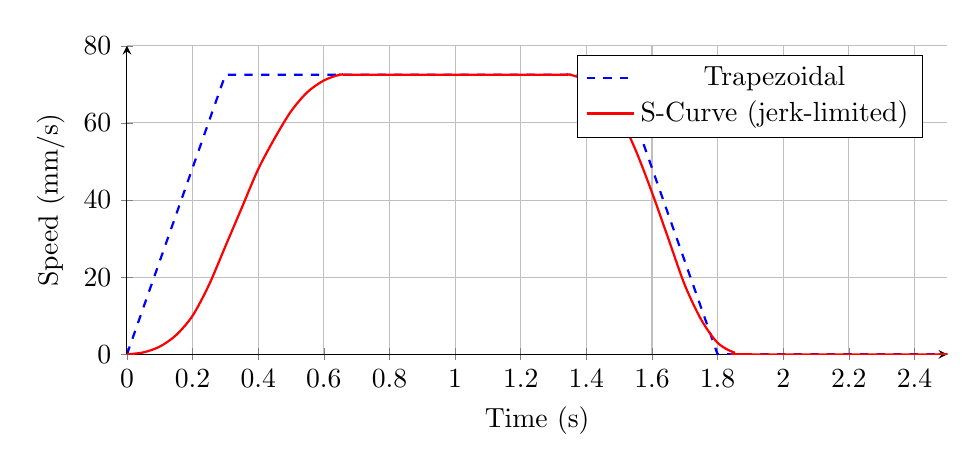
\begin{tikzpicture}
        \begin{axis}[
            width=12cm, height=5.5cm,
            xlabel={Time (s)},
            ylabel={Speed (mm/s)},
            xmin=0, xmax=2.5,
            ymin=0, ymax=80,
            grid=major,
            legend pos=north east,
            axis lines=left,
            domain=0:2.5,
            samples=200
        ]
        % Trapezoidal profile (comparison)
        \addplot[blue, dashed, thick] coordinates {
            (0,0) (0.3,72.5) (1.5,72.5) (1.8,0) (2.5,0)
        };
        % S-curve profile (approximation)
        \addplot[red, thick, smooth] coordinates {
            (0,0) (0.05,0.5) (0.1,2) (0.15,5) (0.2,10) (0.25,18) (0.3,28)
            (0.35,38) (0.4,48) (0.45,56) (0.5,63) (0.55,68) (0.6,71) (0.65,72.5)
            (0.7,72.5) (1.3,72.5) (1.35,72.5) (1.4,71) (1.45,68)
            (1.5,62) (1.55,53) (1.6,42) (1.65,30) (1.7,18) (1.75,9)
            (1.8,3) (1.85,0.5) (1.9,0) (2.5,0)
        };
        \legend{Trapezoidal, S-Curve (jerk-limited)}
        \end{axis}
    \end{tikzpicture}
    \caption{Comparison of trapezoidal and S-curve velocity profiles. The S-curve profile eliminates the discontinuities in acceleration that cause wheel slip and mechanical vibration on low-cost hardware.}
    \label{fig:scurve}
\end{figure}

\subsection{Velocity and Acceleration Feedforward}

The S-curve profiler generates not only the target velocity but also the current acceleration, which is used for \textbf{feedforward compensation}. The feedforward terms pre-compensate for inertia and friction, reducing tracking lag in the closed-loop controller:

\begin{equation}
    v_{\text{ff}} = K_v \cdot v(t) + K_a \cdot a(t)
\end{equation}

\noindent where $K_v = 0.02$ and $K_a = 0.04$ are empirically tuned gains. The feedforward is computed in world frame by the motion queue but must be projected into the robot's \textbf{heading frame} using the inverse rotation transform:

\begin{align}
    V_{\text{ff}} &= \frac{v_{\text{ff},x} \cos\theta - v_{\text{ff},y} \sin\theta}{v_{\max}} \\
    H_{\text{ff}} &= \frac{v_{\text{ff},x} \sin\theta + v_{\text{ff},y} \cos\theta}{v_{\max}}
\end{align}

\noindent Note the use of the \emph{inverse} (transpose) rotation matrix rather than the forward rotation. This subtlety is critical: the feedforward compensates for world-frame inertia, which must be projected \emph{into} the robot frame for correct motor drive computation.

\subsection{Adaptive Lookahead}

The steering algorithm uses an \textbf{adaptive lookahead} that scales with the robot's current speed:

\begin{equation}
    t_{\text{lookahead}} = \text{clamp}\!\left(t_{\text{base}} + v \cdot k_{\text{gain}},\; t_{\min},\; t_{\max}\right)
\end{equation}

\noindent with $t_{\text{base}} = \SI{0.06}{\second}$, $k_{\text{gain}} = 0.0022$, $t_{\min} = \SI{0.04}{\second}$, and $t_{\max} = \SI{0.18}{\second}$.

At high speeds, the extended lookahead accounts for greater momentum and prevents oscillatory tracking. At low speeds near the target, the shortened lookahead provides tighter control for precision positioning. This is substantially more effective than a fixed lookahead, which must compromise between stability at speed and responsiveness at rest.

\subsection{Predictive Braking}
\label{sec:pred-braking}

The robot implements a \textbf{physics-based overshoot prevention} mechanism. At each control tick, it computes the maximum safe entry speed for the remaining distance assuming a fixed deceleration capability:

\begin{equation}
    v_{\text{safe}} = \sqrt{2 \cdot a_{\text{decel}} \cdot d_{\text{remaining}}}
    \label{eq:vsafe}
\end{equation}

\noindent where $a_{\text{decel}} = \SI{350}{mm/s^2}$ and a $1.2\times$ safety margin is applied. If the current closing speed exceeds $v_{\text{safe}}$, the velocity scale is proactively reduced. This prevents the common failure mode where a robot approaches a waypoint too fast, overshoots, turns around, overshoots again, and oscillates indefinitely.

\subsection{Latency-Aware Speed Governor}

A complementary mechanism addresses the specific problem of \textbf{network latency}: when the phone sends a ``stop'' or ``new waypoint'' command, the robot may not receive it for {$\sim$\SI{150}{\milli\second}}. During this window, the robot continues at its current speed and may overshoot. The latency-aware governor imposes a hard upper bound on commanded speed:

\begin{equation}
    v_{\text{cap}} = \sqrt{2 \cdot a_{\text{latency}} \cdot d_{\text{remaining}}}
\end{equation}

\noindent where $a_{\text{latency}} = \SI{300}{mm/s^2}$ (more conservative than the predictive brake). This ensures the robot can always stop within the remaining distance, even if the next command is delayed by a full network round-trip.

\subsection{Blended Angle Stabilization}

During waypoint navigation, the robot must maintain a target heading while translating. A na\"ive approach would use either the internal dead-reckoning angle (which drifts) or the camera ground-truth angle (which arrives sporadically and can jump). Either choice causes problems: DR drift leads to systematic heading error, while camera jumps translate into ``strafe-jumps'' where the heading-frame velocity transform suddenly shifts the motor outputs.

The Pineapple-Bot-Pro solves this with a \textbf{Blended Angle}: an EMA (Exponential Moving Average) fusion of the high-frequency DR angle with the low-frequency camera ground-truth angle. This provides a heading reference that is:

\begin{itemize}
    \item \textbf{Smooth}: The EMA prevents discontinuities from camera observations.
    \item \textbf{Accurate}: The blend converges toward ground truth over time.
    \item \textbf{Responsive}: The high-frequency DR component tracks fast rotations between camera updates.
\end{itemize}

The blended angle is used for both the PID heading stabilization loop and the heading-frame velocity transform, ensuring that corrections from the tracker do not translate into jerky lateral movements.

% ============================================================================
\section{Motor Kinematics and Actuation}
\label{sec:motors}
% ============================================================================

\subsection{Mecanum Drive Model}

The four-motor mecanum drive converts world-frame velocity commands $(v_x, v_y, \omega)$ into individual motor duties. The kinematic model first transforms world-frame velocities into the robot's heading frame using the blended angle $\theta$:

\begin{align}
    V &= \frac{v_x \cos\theta + v_y \sin\theta}{v_{\max}} & \text{(forward/backward)} \\
    H &= \frac{v_x \sin\theta - v_y \cos\theta}{v_{\max}} & \text{(strafe left/right)}
\end{align}

The H-axis output is scaled by $1/\sqrt{2} \approx 0.707$ to normalize the mecanum geometry, which naturally produces $\sqrt{2}\times$ faster strafe than forward motion. The individual motor speeds follow the standard mecanum formula:

\begin{align}
    m_1 &= -H - V - A & \text{(Front Right)} \\
    m_2 &= -H + V - A & \text{Front Left} \\
    m_3 &= -H + V + A & \text{(Back Left)} \\
    m_4 &= -H - V + A & \text{(Back Right)}
\end{align}

\noindent where $A = -\omega / \omega_{\max}$ is the normalized angular velocity.

\subsection{Dead Zone Compensation and Linear Calibration}

Low-cost brushed motors exhibit a significant \textbf{dead zone}---a range of duty cycles too low to overcome static friction. The firmware bypasses this nonlinearity with a calibrated linear mapping:

\begin{equation}
    \text{duty} = 43.017 \cdot |\text{speed}| + 57.165 \cdot \text{sign}(\text{speed})
\end{equation}

\noindent This mapping was determined empirically by plotting commanded duty vs.\ measured wheel velocity, fitting a linear regression, and extracting the slope (\SI{43.017}{}) and offset (\SI{57.165}{}). The offset term ensures that any nonzero speed command immediately jumps past the dead zone.

\subsection{Torque Balancing}

Physical measurement revealed that the right-side motors (M1, M4) produce more torque than the left-side motors (M2, M3), likely due to manufacturing variability in the low-cost motors. Without compensation, this imbalance causes the robot to veer during straight-line motion, degrading dead-reckoning accuracy.

The firmware applies a fixed \textbf{duty reduction of $-3.0$} to the right-side motors, with a lower clamp of $0.5\times$ \texttt{DRIVE\_CLAMP\_LOW} to prevent the reduction from stopping a motor entirely. This simple calibration corrects the systematic drift.

\subsection{Kickstart Mechanism}

Low-cost brushed motors have high static friction relative to kinetic friction. When a motor transitions from stationary to moving, the initial PWM duty may be insufficient to break static hold, causing a brief stall. The \textbf{Kickstart} mechanism addresses this by applying an elevated duty (nominally $70$) for \textbf{3~control frames} (\SI{3}{\milli\second} at \SI{1}{\kilo\hertz}) whenever a motor abruptly transitions from zero speed to nonzero speed. The boost is proportional to the target speed to prevent overshoot during slow manoeuvres.

\subsection{Operating Modes}

The motor controller dynamically selects among three operating modes based on the robot's proximity to its target:

\subsubsection{Normal Mode ($> \SI{50}{\milli\metre}$ from target)}

Standard mecanum control with kickstart, dead zone compensation, and torque balancing. The duty floor is \texttt{DRIVE\_CLAMP\_LOW} = 65.

\subsubsection{Precision Mode ($< \SI{50}{\milli\metre}$ from target)}
\label{sec:precision}

When within \SI{50}{\milli\metre} of the target, the robot enters \textbf{Precision Mode} with a specialized \textbf{Induction Kickstart}. Unlike the standard kickstart (which always fires), the induction kickstart is \emph{conditional}: it activates only when the motors are stalled---defined as commanded speed $> 0.05$ while observed speed $< \SI{1.5}{mm/s}$. If the robot is already moving, the boost is suppressed to prevent the oscillatory ``wiggle'' that occurs when repeated kickstarts fight the precision corrections.

The \textbf{Settling Band} ($< \SI{20}{\milli\metre}$) uses a linear ramp-to-zero duty rather than a fixed floor, allowing the motors to produce arbitrarily small forces for the final approach.

\subsubsection{Single-Motor Mode ($< \SI{15}{\milli\metre}$ from target, $< \SI{10}{mm/s}$)}
\label{sec:single-motor}

This is a novel operating mode designed for \textbf{extreme micro-adjustments}. When within \SI{15}{\milli\metre} of the target and moving slowly, the firmware activates only \emph{one} wheel at a time, producing the smallest possible robot displacement ({$\sim$1--2\,mm} per step).

The wheel selection uses a \textbf{dot-product alignment} algorithm:

\begin{enumerate}
    \item Compute the unit velocity vector in the desired direction: $\hat{\mathbf{d}} = (d_x, d_y)$.
    \item For each mecanum wheel $i$, compute the dot product of $\hat{\mathbf{d}}$ with the wheel's velocity contribution vector $\hat{\mathbf{w}}_i$.
    \item Select the wheel with the largest positive dot product (most aligned with the desired direction).
    \item Drive that single wheel at a conservative fixed duty (\texttt{DRIVE\_CLAMP\_LOW} + 5 = 70).
\end{enumerate}

The wheel velocity vectors for the standard mecanum layout are:

\begin{align}
    \hat{\mathbf{w}}_1 &= (-1, -1)/\sqrt{2} & \text{(Front Right)} \\
    \hat{\mathbf{w}}_2 &= (-1, +1)/\sqrt{2} & \text{(Back Right)} \\
    \hat{\mathbf{w}}_3 &= (+1, +1)/\sqrt{2} & \text{(Back Left)} \\
    \hat{\mathbf{w}}_4 &= (+1, -1)/\sqrt{2} & \text{(Front Left)}
\end{align}

By firing only the most-aligned wheel, the robot avoids introducing parasitic rotation (which all four-wheel actuation inevitably creates due to imperfect motor matching) and achieves displacements far below what the standard mecanum formula can reliably produce.

\subsection{Anti-Slip and Stall Detection}

Despite the traction analysis presented in \Cref{sec:hardware}, wheel slip can still occur on contaminated surfaces or when the robot's weight shifts during servo actuation. The firmware implements a \textbf{stall detector} that monitors the discrepancy between commanded and observed velocity:

\begin{itemize}
    \item \textbf{Trigger condition:} Observed velocity $< \SI{5}{mm/s}$ while commanded speed $> \SI{20}{mm/s}$ for \textbf{75 consecutive control ticks} (\SI{75}{\milli\second}).
    \item \textbf{Response:} Apply a $1.35\times$ multiplicative duty boost to all motors for up to 100 ticks.
\end{itemize}

The detection requires sustained stall (75 ticks) rather than instantaneous detection to avoid false triggers during normal deceleration, where the commanded speed briefly exceeds the observed speed as the S-curve ramps down.

\subsection{Active Braking (Reverse Thrust)}

When a motion segment ends, physical momentum causes the robot to coast past the target. The firmware applies \textbf{active reverse thrust} to kill this momentum:

\begin{itemize}
    \item \textbf{Rotation braking:} Reverse duty 75 for \SI{15}{\milli\second} (15 control ticks), triggered when the prior motion was rotation-only and the angular velocity exceeded \SI{5}{deg/s}.
    \item \textbf{Translation braking:} Reverse duty 80 for \SI{18}{\milli\second} (18 control ticks), triggered when the observed speed exceeds \SI{5}{mm/s}. The reverse thrust direction is computed from the Kalman-estimated velocity vector, projected into the robot's heading frame.
\end{itemize}

Translation braking is \textbf{suppressed during HOLDING state} to prevent oscillation: the HOLDING corrections are intentionally small, and applying reverse thrust after each one would cause the robot to oscillate back and forth around the target.

\subsection{Drift Trim}

Empirical testing revealed a systematic lateral drift during forward motion, attributed to manufacturing asymmetries in the mecanum rollers. The firmware pre-rotates the $(V, H)$ velocity vector by a calibrated \textbf{drift trim angle} before applying it to the motors. The trim is speed-dependent:

\begin{table}[H]
    \centering
    \caption{Drift trim calibration values (Robot A).}
    \label{tab:drift-trim}
    \begin{tabular}{@{}ll@{}}
        \toprule
        \textbf{Speed Level} & \textbf{Trim Angle} \\
        \midrule
        SLOW   & $9.36°$ \\
        NORMAL & $0.00°$ \\
        FAST   & $0.00°$ \\
        \bottomrule
    \end{tabular}
\end{table}

\subsection{Motor Duty Normalization}

If the combined effects of translation, rotation, and feedforward produce motor duties exceeding the hardware maximum (\texttt{DRIVE\_CLAMP\_HIGH} = 100), all four motor duties are proportionally scaled down to fit within the limit. This preserves the intended velocity direction and rotation ratio while preventing saturation.

% ============================================================================
\section{Dead Reckoning and Latency-Compensated Vision}
\label{sec:dr}
% ============================================================================

\subsection{Dead Reckoning Engine}

The \texttt{DeadReckoning} subsystem integrates commanded velocities at each \SI{1}{\milli\second} control loop tick to maintain a continuous position estimate. It employs a \textbf{two-tier position model}:

\begin{enumerate}
    \item \textbf{Internal Odometer} $(\text{ix}, \text{iy}, \text{ia})$: Continuously integrated from velocity. Never resets except at startup.
    \item \textbf{Global Anchor} $(\text{gx}, \text{gy}, \text{ga})$: Absolute correction from camera observations. Set by the latency compensator.
\end{enumerate}

The current best-estimate position is computed as:

\begin{equation}
    \mathbf{p}_{\text{current}} = \mathbf{p}_{\text{anchor}} + (\mathbf{p}_{\text{odometer}} - \mathbf{p}_{\text{odometer@anchor}})
    \label{eq:dr-model}
\end{equation}

This model separates the accumulated error (captured in the anchor offset) from the incremental tracking (which remains accurate over short intervals), enabling smooth camera corrections without disrupting the odometric continuity.

\subsubsection{Distance Calibration}

Dead reckoning accuracy depends critically on the mapping between commanded velocity and actual displacement. The firmware applies empirically calibrated \textbf{distance factors}: $1.0 \times$ for vertical (forward/backward) and $1.25 \times$ for horizontal (strafe) motion on Robot~A. The horizontal factor reflects the $\sim 20\%$ systematic under-travel inherent to mecanum strafing, where roller slip dissipates a fraction of the commanded displacement.

\subsubsection{EMA-Smoothed Velocity for Integration}

A subtle but important detail: the dead reckoning uses an \textbf{EMA-smoothed} commanded velocity rather than the instantaneous value for integration. When the motion queue's speed scale drops to zero (segment end), the raw velocity falls to zero instantly, but the robot physically coasts for \SI{\sim 30}{\milli\second}. The EMA velocity decays naturally over this period, keeping the DR position estimate accurate through the coasting phase.

\subsubsection{Position History Ring Buffer}

The engine maintains a \textbf{ring buffer of 256 position snapshots}, each recording the internal odometer state and timestamp. This buffer is protected by a dedicated FreeRTOS mutex (separate from the main state mutex) to allow Core~0 to query historical positions during camera update processing without blocking Core~1's control loop. The latency compensator uses this buffer to look up ``where did the robot think it was at the moment the camera frame was captured?''

\subsection{Kalman-Filtered Velocity Estimation}
\label{sec:kalman}

Instantaneous velocity computed from position differences is noisy, especially at \SI{1}{\kilo\hertz} where quantization effects dominate. The motion queue employs a \textbf{1D Kalman filter per axis} (X and Y independently) with a position-velocity state model:

\begin{equation}
    \mathbf{x}_k = \begin{bmatrix} p \\ v \end{bmatrix}, \quad
    \mathbf{F} = \begin{bmatrix} 1 & \Delta t \\ 0 & 1 \end{bmatrix}, \quad
    \mathbf{H} = \begin{bmatrix} 1 & 0 \end{bmatrix}
\end{equation}

The filter parameters are:

\begin{table}[H]
    \centering
    \caption{Kalman filter noise parameters.}
    \label{tab:kalman-params}
    \begin{tabular}{@{}lll@{}}
        \toprule
        \textbf{Parameter} & \textbf{Symbol} & \textbf{Value} \\
        \midrule
        Process noise (position) & $q_p$ & 0.5 \\
        Process noise (velocity) & $q_v$ & 50.0 \\
        Measurement noise        & $r$   & 2.0 \\
        \bottomrule
    \end{tabular}
\end{table}

The relatively high process noise for velocity ($q_v = 50.0$) allows the filter to track rapid velocity changes (as commanded by the S-curve profiler) while still rejecting noise.

A \textbf{Stationary Deadzone} of \SI{5.0}{mm/s} is applied to the Kalman velocity estimate: if the estimated speed falls below this threshold, it is clamped to zero. This prevents stale velocity signals from influencing the braking logic when the robot is nominally stationary but the Kalman filter has not yet fully converged to zero.

\subsection{Clock Synchronization}

The robot and phone operate on independent clocks with different origins and potential drift. The system achieves millisecond-level synchronization through a \textbf{PING/PONG protocol}:

\begin{enumerate}
    \item The robot sends \texttt{P:\{robot\_timestamp\}} every \SI{500}{\milli\second}.
    \item The phone replies with \texttt{Q:\{robot\_timestamp\}:\{phone\_timestamp\}}.
    \item The robot computes the round-trip time (RTT) using an exponential moving average ($\alpha = 1/8$) and derives the clock offset: $\Delta_{\text{clock}} = t_{\text{phone}} - t_{\text{robot}} - \text{RTT}/2$.
\end{enumerate}

This clock offset is essential for the latency compensator to correctly timestamp camera observations in the robot's time domain.

\subsection{Latency-Compensated Vision}
\label{sec:latency-comp}

The smartphone camera introduces an inherent {$\sim$\SI{150}{\milli\second}} latency between frame capture and the arrival of the processed position observation at the robot. Na\"ively applying this observation as a direct position correction would cause the robot to ``jump back'' to where it was \SI{150}{\milli\second} ago, creating oscillatory behavior.

The \textbf{Latency Compensator} solves this with a retroactive correction algorithm:

\begin{enumerate}
    \item When a camera update \texttt{C:\{ts\}:\{x\}:\{y\}:\{angle\}} arrives, the compensator converts the phone timestamp $t_{\text{phone}}$ to robot time using the synchronized clock offset, and subtracts the assumed camera processing latency (\SI{150}{\milli\second}).

    \item It queries the dead-reckoning history buffer (\Cref{sec:dr}) to find the odometric state at the \emph{capture instant}: ``Where did the robot think it was when this frame was taken?''

    \item The difference between the camera observation and the historical position estimate is the \textbf{measured drift}:
    \begin{equation}
        \mathbf{e}_{\text{drift}} = \mathbf{p}_{\text{camera}} - \mathbf{p}_{\text{DR@capture}}
    \end{equation}

    \item If $\|\mathbf{e}_{\text{drift}}\| > \SI{5.0}{\milli\metre}$ (the drift threshold), a correction is triggered. The drift error is blended forward into the current position estimate over a \SI{200}{\milli\second} interpolation window using a smooth correction policy, preventing jarring jumps.

    \item If $\|\mathbf{e}_{\text{drift}}\| > \SI{25.0}{\milli\metre}$ (the emergency threshold), an immediate correction is applied to prevent the robot from operating on a grossly incorrect position belief.
\end{enumerate}

\begin{figure}[H]
    \centering
    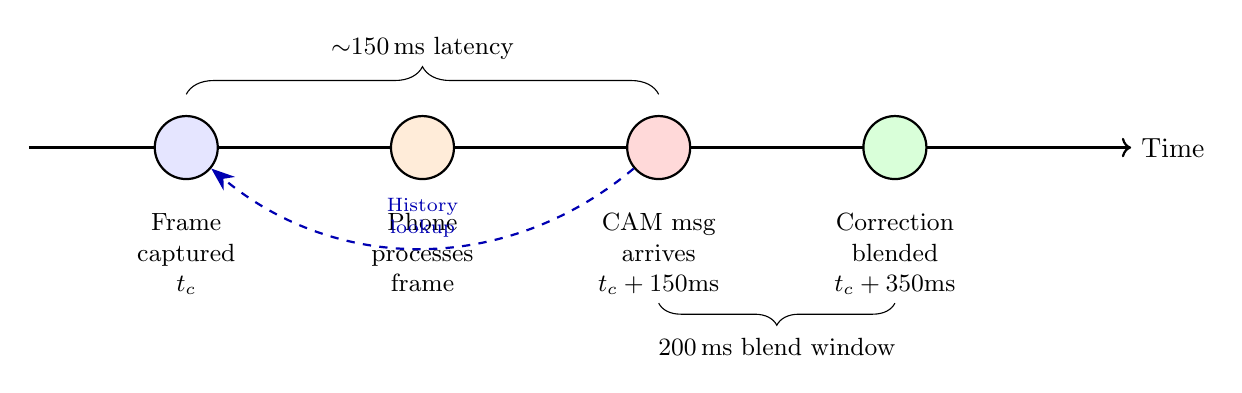
\begin{tikzpicture}[
        event/.style={circle, draw, thick, fill=blue!10, minimum size=0.8cm, font=\small},
        label/.style={font=\small, align=center},
        arrow/.style={-{Stealth[length=3mm]}, thick}
    ]
        % Timeline
        \draw[thick, ->] (0,0) -- (14,0) node[right] {Time};

        % Events
        \node[event] (cap) at (2,0) {};
        \node[label, below=0.3cm of cap] {Frame\\captured\\$t_c$};

        \node[event, fill=orange!15] (proc) at (5,0) {};
        \node[label, below=0.3cm of proc] {Phone\\processes\\frame};

        \node[event, fill=red!15] (arrive) at (8,0) {};
        \node[label, below=0.3cm of arrive] {CAM msg\\arrives\\$t_c + 150\text{ms}$};

        \node[event, fill=green!15] (correct) at (11,0) {};
        \node[label, below=0.3cm of correct] {Correction\\blended\\$t_c + 350\text{ms}$};

        % Latency bracket
        \draw[decorate, decoration={brace, amplitude=10pt, raise=5pt}] (2,0.5) -- (8,0.5) node[midway, above=0.5cm, font=\small] {$\sim$150\,ms latency};

        % Blend bracket
        \draw[decorate, decoration={brace, amplitude=8pt, raise=5pt, mirror}] (8,-1.8) -- (11,-1.8) node[midway, below=0.5cm, font=\small] {200\,ms blend window};

        % History lookup
        \draw[arrow, dashed, blue!70!black] (arrive) to[bend left=40] node[above, font=\scriptsize, align=center] {History\\lookup} (cap);
    \end{tikzpicture}
    \caption{Latency compensation timeline. When a camera observation arrives at $t_c + 150\text{ms}$, the compensator looks up the dead-reckoning state at $t_c$ (the actual capture time), computes the drift error, and blends the correction over a \SI{200}{\milli\second} window to prevent position jumps.}
    \label{fig:latency-comp}
\end{figure}

\subsection{Heading Authority}

For heading stabilization during translation, the controller must choose between the dead-reckoning angle (high frequency, but drifts) and the camera angle (accurate, but low frequency and prone to jumps). As described in \Cref{sec:motion}, the \textbf{Blended Angle}---an EMA fusion of both sources---provides the best of both worlds. This blended angle serves as the \emph{heading authority} for:

\begin{itemize}
    \item The PID heading stabilization loop (computing heading error)
    \item The heading-frame velocity transform (projecting world-frame velocities into the robot frame)
    \item The feedforward projection (transforming world-frame acceleration into the robot frame)
\end{itemize}

% ============================================================================
\section{Android Controller Application}
\label{sec:android}
% ============================================================================

The Android companion application (\texttt{PineappleRobotPro}) serves three roles: external vision system, mission controller, and real-time telemetry display. It is implemented in Kotlin with Jetpack Compose for the UI layer.

\subsection{Architecture Overview}

The application is decomposed into the following components:

\begin{table}[H]
    \centering
    \caption{Android application component architecture.}
    \label{tab:android-components}
    \begin{tabularx}{\textwidth}{@{}lXl@{}}
        \toprule
        \textbf{Component} & \textbf{Responsibility} & \textbf{Size} \\
        \midrule
        \texttt{MainActivity}    & UI composition, state management, camera frame processing, path editor & \SI{75}{\kilo\byte} \\
        \texttt{UIComponents}    & Reusable Compose UI elements: field view, robot overlays, control panels & \SI{98}{\kilo\byte} \\
        \texttt{RobotUdpBridge}  & UDP communication, robot discovery, tap-target and heading-lock control loops & \SI{31}{\kilo\byte} \\
        \texttt{CameraComponents} & CameraX integration, perspective warp, ArUco detection via OpenCV & \SI{15}{\kilo\byte} \\
        \texttt{ContinuousMotionController} & Multi-waypoint path sequencer, servo action scheduling & \SI{11}{\kilo\byte} \\
        \texttt{DataModels}      & Protocol enums, path graph data structures, field constants & \SI{5}{\kilo\byte} \\
        \texttt{StorageHelpers}  & Configuration persistence, path serialization & \SI{22}{\kilo\byte} \\
        \texttt{NavigationHistoryManager} & Undo/redo for path editing operations & \SI{2}{\kilo\byte} \\
        \bottomrule
    \end{tabularx}
\end{table}

\subsection{Vision Pipeline}

The vision pipeline transforms raw camera frames into robot position observations:

\begin{enumerate}
    \item \textbf{Frame Capture:} CameraX provides frames at the device's native rate (typically \SI{30}{\hertz}) in RGBA format. The app preferentially selects the \textbf{ultra-wide lens} (focal length $< \SI{2.5}{\milli\metre}$) to maximize the field of view.

    \item \textbf{Perspective Warp:} Four user-calibrated corner points define the playing field boundary. A perspective transform (\texttt{Imgproc.getPerspectiveTransform}) warps the captured frame into a rectified top-down view of the field. The transform accounts for:
    \begin{itemize}
        \item A configurable padding region around the field boundary to track robots that have moved slightly outside the playing area
        \item The field's aspect ratio ($\SI{1143}{\milli\metre} \times \SI{1181}{\milli\metre}$)
    \end{itemize}

    \item \textbf{ArUco Detection:} The warped, grayscale image is processed by OpenCV's \texttt{ArucoDetector} using a 4$\times$4 dictionary (50 markers). Each robot carries a unique ArUco marker (ID~0 for Robot~A, ID~1 for Robot~B).

    \item \textbf{Pose Extraction:} For each detected marker, the center position is computed as the mean of the four corner coordinates (normalized to the field boundary), and the heading angle is extracted from the vector between the top and bottom edge midpoints:

    \begin{equation}
        \theta = \text{atan2}\!\left(-\Delta_y,\; \Delta_x\right) \cdot \frac{180^\circ}{\pi}
    \end{equation}

    The use of ArUco marker detection is a standard technique and is not claimed as a contribution; rather, it serves as a reliable, zero-cost fiducial system that integrates well with the OpenCV library already required for perspective warping.

    \item \textbf{Coordinate Transform:} Normalized marker positions are scaled to millimetres using the known field dimensions and transmitted to the robot as \texttt{CAM} messages with the capture timestamp.
\end{enumerate}

\subsection{Robot Discovery and Connection}

The \texttt{RobotUdpBridge} implements an \textbf{automatic discovery protocol}:

\begin{enumerate}
    \item The app listens on UDP port 4210 for incoming packets.
    \item When a robot sends a \texttt{HELLO} or \texttt{REGISTER} message, the bridge records the robot's ID, IP address, and last-seen timestamp.
    \item Robots are considered connected if their last-seen time is within \SI{10}{\second}.
    \item All subsequent commands are routed to the robot by ID, with the IP address resolved from the registry.
\end{enumerate}

This design supports \textbf{multi-robot operation}: multiple robots can connect simultaneously, each identified by its unique ID (``A'', ``B''). The phone broadcasts camera observations to all visible robots and routes commands per-robot.

\subsection{Tap-Target Navigation}

The app implements a \textbf{Tap-Target} control mode where the user taps a position on the field view, and the app autonomously navigates the robot to that location. The tap-target controller operates as a periodic feedback loop:

\begin{enumerate}
    \item On each camera update, the controller checks if the robot is within the arrival tolerance (X: \SI{10}{\milli\metre}, Y: \SI{15}{\milli\metre}, angle: $4^\circ$).
    \item If outside tolerance, it sends a \texttt{WAYPOINT} command to the robot at a rate governed by a \textbf{distance-based cooldown}:
    \begin{itemize}
        \item $> \SI{150}{\milli\metre}$: \SI{100}{\milli\second} cooldown (fast updates)
        \item 80--\SI{150}{\milli\metre}: \SI{160}{\milli\second}
        \item 40--\SI{80}{\milli\metre}: \SI{250}{\milli\second}
        \item $<$ \SI{40}{\milli\metre}: \SI{400}{\milli\second} (precision pulsing)
    \end{itemize}
    \item Arrival is confirmed only after \textbf{3 consecutive stable frames} within tolerance, preventing premature declaration when the robot passes through the target while overshooting.
\end{enumerate}

The asymmetric X/Y tolerances ($\SI{10}{\milli\metre}$ vs.\ $\SI{15}{\milli\metre}$) account for the inherent difficulty of mecanum control in the forward/backward axis versus strafe.

\subsection{Path Sequencer (Continuous Motion Controller)}

For autonomous mission execution, the app implements a \textbf{Continuous Motion Controller} that sequences multi-waypoint paths:

\begin{enumerate}
    \item A course is defined as an ordered list of \texttt{Waypoint} objects, each specifying a position, heading, tolerances, and optional servo actions.
    \item The sequencer navigates to each waypoint in order by delegating to the tap-target system.
    \item Upon arrival at each waypoint, the sequencer executes any associated servo actions sequentially, waiting \SI{800}{\milli\second} between actions.
    \item After all servo actions complete, the sequencer advances to the next waypoint.
    \item The sequencer supports \textbf{cross-robot wait conditions}: a waypoint can specify that it should not be started until a different robot has reached a specific node, enabling coordinated multi-robot missions.
\end{enumerate}

\subsection{Graph-Based Path Editor}

The app includes a visual path editor that allows users to design robot courses directly on the warped field view:

\begin{itemize}
    \item \textbf{Node Placement:} Tap to place nodes at specific field coordinates.
    \item \textbf{Connection Management:} Draw connections between nodes to define traversal order.
    \item \textbf{Per-Node Configuration:} Set rotation angle, servo actions (two slots per node), tolerances, and cross-robot wait conditions.
    \item \textbf{Fruit Detection Integration:} Nodes can reference specific fruit positions from a hard-coded grid, with the app automatically determining the appropriate servo action based on detected fruit color (red, green, or absent).
    \item \textbf{Undo/Redo:} Full undo/redo support via the \texttt{NavigationHistoryManager}.
    \item \textbf{Persistence:} Paths are serialized and persisted to device storage, surviving app restarts.
\end{itemize}

% ============================================================================
\section{Integrated Control Flow}
\label{sec:control-flow}
% ============================================================================

The complete control flow from camera observation to motor actuation spans both platforms and multiple algorithmic stages. \Cref{fig:control-flow} illustrates the end-to-end pipeline.

\begin{figure}[H]
    \centering
    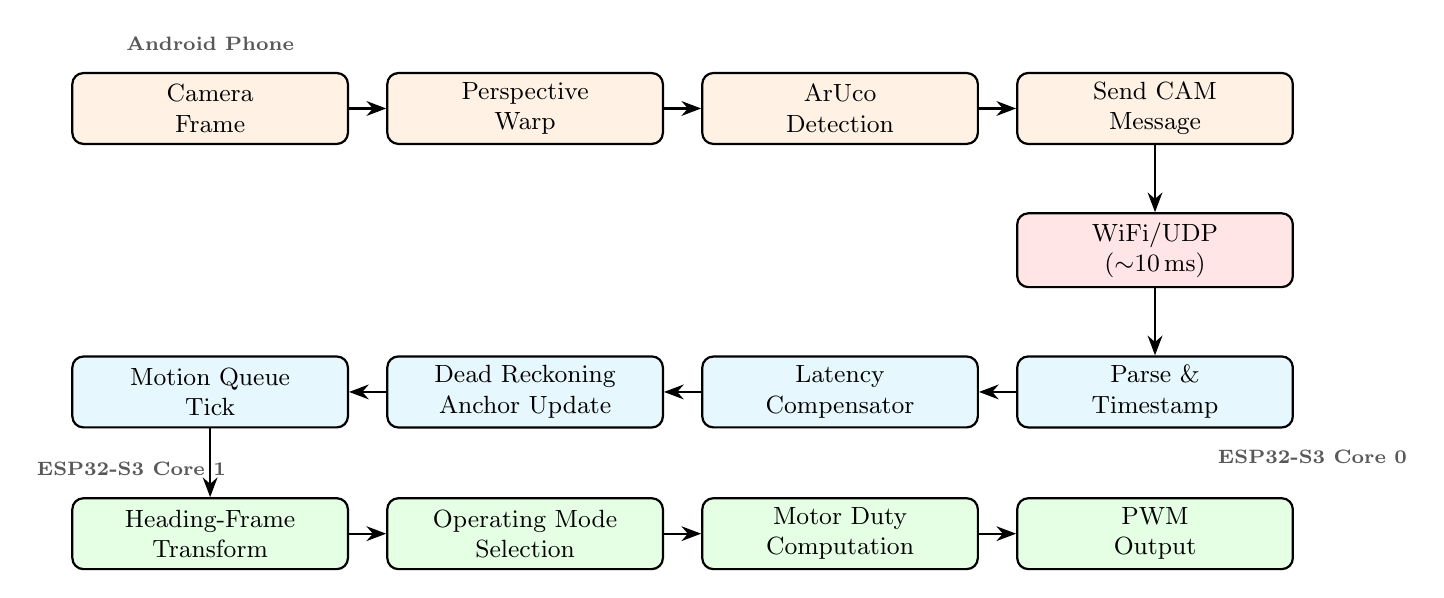
\begin{tikzpicture}[
        stage/.style={rectangle, draw, rounded corners, thick, minimum height=0.9cm, minimum width=3.5cm, align=center, font=\small, fill=#1},
        arrow/.style={-{Stealth[length=2.5mm]}, thick},
        note/.style={font=\scriptsize, align=center, text=gray!70!black}
    ]
        % Phone stages
        \node[stage=orange!10] (camera) at (0, 0) {Camera\\Frame};
        \node[stage=orange!10] (warp) at (4, 0) {Perspective\\Warp};
        \node[stage=orange!10] (aruco) at (8, 0) {ArUco\\Detection};
        \node[stage=orange!10] (send) at (12, 0) {Send CAM\\Message};

        % Network
        \node[stage=red!10] (network) at (12, -1.8) {WiFi/UDP\\({$\sim$10\,ms})};

        % Robot stages
        \node[stage=cyan!10] (parse) at (12, -3.6) {Parse \&\\Timestamp};
        \node[stage=cyan!10] (lc) at (8, -3.6) {Latency\\Compensator};
        \node[stage=cyan!10] (dr) at (4, -3.6) {Dead Reckoning\\Anchor Update};
        \node[stage=cyan!10] (mq) at (0, -3.6) {Motion Queue\\Tick};

        \node[stage=green!10] (heading) at (0, -5.4) {Heading-Frame\\Transform};
        \node[stage=green!10] (mode) at (4, -5.4) {Operating Mode\\Selection};
        \node[stage=green!10] (duty) at (8, -5.4) {Motor Duty\\Computation};
        \node[stage=green!10] (motors) at (12, -5.4) {PWM\\Output};

        % Arrows
        \draw[arrow] (camera) -- (warp);
        \draw[arrow] (warp) -- (aruco);
        \draw[arrow] (aruco) -- (send);
        \draw[arrow] (send) -- (network);
        \draw[arrow] (network) -- (parse);
        \draw[arrow] (parse) -- (lc);
        \draw[arrow] (lc) -- (dr);
        \draw[arrow] (dr) -- (mq);
        \draw[arrow] (mq) -- (heading);
        \draw[arrow] (heading) -- (mode);
        \draw[arrow] (mode) -- (duty);
        \draw[arrow] (duty) -- (motors);

        % Labels
        \node[note, above=0.15cm of camera] {\textbf{Android Phone}};
        \node[note, below=0.15cm of parse, xshift=2cm] {\textbf{ESP32-S3 Core 0}};
        \node[note, above=0.15cm of heading, xshift=-1cm] {\textbf{ESP32-S3 Core 1}};
    \end{tikzpicture}
    \caption{End-to-end control flow from camera capture to motor actuation. The pipeline spans the phone (camera processing), the network (UDP), Core~0 (parsing), and Core~1 (motion control).}
    \label{fig:control-flow}
\end{figure}

The complete pipeline latency from frame capture to motor response is approximately:

\begin{table}[H]
    \centering
    \caption{Pipeline latency breakdown.}
    \label{tab:latency}
    \begin{tabular}{@{}lr@{}}
        \toprule
        \textbf{Stage} & \textbf{Latency} \\
        \midrule
        Camera capture + CameraX pipeline & {$\sim$\SI{33}{\milli\second}} (at \SI{30}{fps}) \\
        Perspective warp + ArUco detection & {$\sim$30--\SI{50}{\milli\second}} \\
        UDP network transit                & {$\sim$5--\SI{20}{\milli\second}} \\
        Firmware parsing + latency comp.   & {$\sim$\SI{1}{\milli\second}} \\
        Control loop tick                  & $\leq$ \SI{1}{\milli\second} \\
        Motor PWM update                   & $<$ \SI{0.1}{\milli\second} \\
        \midrule
        \textbf{Total (estimated)}         & {$\sim$70--\SI{105}{\milli\second}} \\
        \textbf{Assumed for compensation}  & \SI{150}{\milli\second} (conservative) \\
        \bottomrule
    \end{tabular}
\end{table}

% ============================================================================
\section{S-Curve Tuning Strategy Across Robot Configurations}
\label{sec:tuning}
% ============================================================================

The physical measurements in \Cref{sec:hardware} reveal a critical constraint: Robot~B's traction limit (\SI{3652}{mm/s^2}) is less than half of Robot~A's (\SI{8308}{mm/s^2}). Since the firmware must produce reliable dead reckoning on both robots without risking wheel slip, the S-curve profiler's operational bounds must be capped below the \textbf{lowest common traction limit} across the fleet.

The current S-curve parameters (peak acceleration \SI{250}{mm/s^2}, peak jerk \SI{1200}{mm/s^3}) are set conservatively below Robot~B's traction limit by a factor of $\sim 14.6\times$. This generous margin accounts for:

\begin{itemize}
    \item Surface variability (the competition field may have different friction characteristics than the calibration surface)
    \item Dynamic weight shifts during servo actuation
    \item The cumulative effect of feedforward compensation, which adds to the commanded acceleration
    \item The asymmetric deceleration limits ($2\times$ acceleration), which bring the peak deceleration to \SI{500}{mm/s^2}---still well within the traction envelope
\end{itemize}

% ============================================================================
\section{Speed Profiles and Operational Parameters}
\label{sec:speed-profiles}
% ============================================================================

The firmware supports three speed levels, each calibrated from PS2 controller physics at 100\% duty:

\begin{table}[H]
    \centering
    \caption{Speed profile calibration values (default, before scaling).}
    \label{tab:speed-profiles}
    \begin{tabular}{@{}lll@{}}
        \toprule
        \textbf{Speed Level} & \textbf{Translation} & \textbf{Rotation} \\
        \midrule
        SLOW   & \SI{29.0}{mm/s}  & \SI{15.0}{deg/s} \\
        NORMAL & \SI{43.5}{mm/s}  & \SI{51.84}{deg/s} \\
        FAST   & \SI{72.5}{mm/s}  & \SI{86.4}{deg/s} \\
        \bottomrule
    \end{tabular}
\end{table}

These values may appear modest compared to larger competition robots, reflecting the deliberately low-cost, low-power drive system. The system compensates for limited speed with high precision: the combination of S-curve profiling, predictive braking, and single-motor micro-adjustments enables the robot to achieve its \SI{5}{\milli\metre} waypoint tolerance consistently despite peak speeds of only \SI{72.5}{mm/s}.

\subsection{Precision Thresholds}

\begin{table}[H]
    \centering
    \caption{Precision control thresholds.}
    \label{tab:precision}
    \begin{tabular}{@{}ll@{}}
        \toprule
        \textbf{Parameter} & \textbf{Value} \\
        \midrule
        Precision mode activation distance  & \SI{50}{\milli\metre} \\
        Single-motor mode activation        & \SI{15}{\milli\metre} \\
        Waypoint arrival tolerance           & \SI{5}{\milli\metre} \\
        Rotation arrival tolerance           & $1.5^\circ$ \\
        Close approach distance             & \SI{120}{\milli\metre} \\
        Waypoint deduplication tolerance     & \SI{15}{\milli\metre} \\
        Heading stabilization gain           & 2.5 \\
        Maximum stabilization $\omega$       & \SI{35}{deg/s} \\
        \bottomrule
    \end{tabular}
\end{table}

% ============================================================================
\section{Discussion}
\label{sec:discussion}
% ============================================================================

\subsection{Novel Contributions}

The Pineapple-Bot-Pro system makes several technical contributions within the context of low-cost educational robotics:

\begin{enumerate}
    \item \textbf{Retroactive Latency Compensation:} Rather than trying to reduce the camera pipeline latency (which is fundamentally limited by smartphone hardware and processing), the system embraces the latency and \emph{compensates retroactively} using the dead-reckoning history buffer. This approach is applicable to any system where observation latency is known and deterministic localization is available between observations.

    \item \textbf{Jerk-Limited S-Curve on a \$3 Microcontroller:} S-curve trajectory profiling is typically associated with industrial motion controllers. Implementing it in a \SI{1}{\kilo\hertz} control loop on an ESP32-S3 demonstrates that the computational requirements are well within the reach of modern low-cost microcontrollers.

    \item \textbf{Single-Motor Micro-Adjustment:} The dot-product wheel selection algorithm for sub-\SI{2}{\milli\metre} position corrections exploits the specific geometry of mecanum drives in a way not commonly described in the educational robotics literature.

    \item \textbf{Blended Angle Stabilization:} The EMA fusion of dead-reckoning and camera angles for heading authority provides a smooth, accurate reference without the complexity of a full sensor fusion framework (e.g., EKF/UKF).

    \item \textbf{Phone-as-Vision-Sensor:} Using a consumer smartphone as both the external vision system and the mission controller eliminates the need for dedicated vision hardware, reducing system cost and setup complexity.
\end{enumerate}

\subsection{Limitations and Future Work}

\begin{itemize}
    \item \textbf{No Encoder Feedback:} The current system relies entirely on open-loop dead reckoning (time $\times$ speed integration) without wheel encoders. Adding encoders would significantly improve DR accuracy and enable closed-loop motor speed control.

    \item \textbf{WiFi Reliability:} The WiFi link is susceptible to interference in crowded competition venues. A dedicated radio link (e.g., ESP-NOW, which uses the same ESP32 hardware) could reduce latency and improve reliability.

    \item \textbf{Camera Frame Rate:} The smartphone camera operates at \SI{30}{fps}, limiting the vision update rate to {$\sim$\SI{30}{\hertz}}. Higher frame rates would improve the blended angle convergence and reduce the reliance on dead reckoning between observations.

    \item \textbf{Single-Axis Kalman Filters:} The per-axis Kalman filters do not model cross-axis coupling. A 4-state coupled filter ($x, y, v_x, v_y$) could improve velocity estimation during diagonal motion.
\end{itemize}

% ============================================================================
\section{Conclusion}
\label{sec:conclusion}
% ============================================================================

This report has presented the Pineapple-Bot-Pro, a low-cost autonomous mecanum-drive robot system designed for the Vietnam Robotics For Good national competition. The system demonstrates that sophisticated autonomous behavior---including jerk-limited trajectory profiling, latency-compensated vision, single-motor micro-adjustments, and multi-robot coordination---can be achieved on commodity hardware costing well under \$50 USD per robot.

The key insight driving the design is that modern low-cost microcontrollers (such as the ESP32-S3) have sufficient computational power to run advanced control algorithms at high frequencies, making software sophistication the most cost-effective path to improved robot performance. The dual-core architecture, running a \SI{1}{\kilo\hertz} control loop alongside asynchronous network processing, enables deterministic motor control while maintaining responsive communication---a capability that would have required dedicated hardware a decade ago.

The system achieves $\pm$\SI{5}{\milli\metre} positional accuracy and $\pm 1.5^\circ$ angular accuracy on a \SI{1143}{\milli\metre} $\times$ \SI{1181}{\milli\metre} competition field, using only a consumer smartphone for external localization. These results validate the design philosophy of investing in algorithmic complexity rather than expensive hardware, and suggest that similar approaches could benefit other resource-constrained robotics applications.

% ============================================================================
% References
% ============================================================================
\newpage
\section*{References}

\begin{enumerate}[label={[\arabic*]}]
    \item Espressif Systems, ``ESP32-S3 Technical Reference Manual,'' Version 1.1, 2022. [Online]. Available: \url{https://www.espressif.com/en/products/socs/esp32-s3}

    \item S.~Garrido-Jurado, R.~Mu\~noz-Salinas, F.~J.~Madrid-Cuevas, and M.~J.~Mar\'in-Jim\'enez, ``Automatic generation and detection of highly reliable fiducial markers under occlusion,'' \textit{Pattern Recognition}, vol.~47, no.~6, pp.~2280--2292, 2014.

    \item R.~Siegwart, I.~R.~Nourbakhsh, and D.~Scaramuzza, \textit{Introduction to Autonomous Mobile Robots}, 2nd~ed. Cambridge, MA: MIT Press, 2011.

    \item G.~Welch and G.~Bishop, ``An Introduction to the Kalman Filter,'' University of North Carolina, Chapel Hill, TR~95-041, 2006.

    \item Tower Pro, ``SG90 Micro Servo Datasheet,'' [Online]. Available: \url{http://www.towerpro.com.tw/product/sg90-7/}

    \item PlatformIO, ``PlatformIO: An open source ecosystem for IoT development,'' [Online]. Available: \url{https://platformio.org/}

    \item OpenCV, ``ArUco Marker Detection,'' OpenCV Documentation. [Online]. Available: \url{https://docs.opencv.org/4.x/d5/dae/tutorial_aruco_detection.html}

    \item R.~A.~Brooks, ``A robust layered control system for a mobile robot,'' \textit{IEEE Journal on Robotics and Automation}, vol.~2, no.~1, pp.~14--23, 1986.
\end{enumerate}

% ============================================================================
% Appendices
% ============================================================================
\newpage
\appendix

\section{Configuration Defaults Reference}
\label{app:config}

\begin{table}[H]
    \centering
    \caption{Complete firmware configuration parameters with default values.}
    \label{tab:full-config}
    \small
    \begin{tabular}{@{}p{5.5cm}ll@{}}
        \toprule
        \textbf{Parameter} & \textbf{Default} & \textbf{Unit} \\
        \midrule
        \multicolumn{3}{@{}l}{\textit{Motor Physics}} \\
        \texttt{DRIVE\_CLAMP\_LOW}          & 65   & duty \\
        \texttt{DRIVE\_CLAMP\_HIGH}         & 100  & duty \\
        \texttt{DRIVE\_CLAMP\_FINE}         & 65   & duty \\
        \texttt{MOTOR\_MAP\_SLOPE}          & 43.017 & --- \\
        \texttt{MOTOR\_MAP\_OFFSET}         & 57.165 & --- \\
        \texttt{KICKSTART\_FRAMES}          & 3    & ticks \\
        \texttt{KICKSTART\_SPEED}           & 70.0 & duty \\
        \texttt{RAMP\_DURATION\_MS}         & 75   & ms \\
        \texttt{RAMP\_START\_FRACTION}      & 0.15 & --- \\
        \midrule
        \multicolumn{3}{@{}l}{\textit{Precision Control}} \\
        \texttt{PRECISION\_MODE\_THRESH\_MM}    & 50   & mm \\
        \texttt{WAYPOINT\_TOLERANCE\_MM}        & 5.0  & mm \\
        \texttt{ROTATION\_TOLERANCE\_DEG}       & 1.5  & deg \\
        \texttt{CLOSE\_APPROACH\_DISTANCE\_MM}  & 120  & mm \\
        \texttt{STABILIZATION\_GAIN}            & 2.5  & --- \\
        \texttt{MAX\_STABILIZATION\_OMEGA}      & 35.0 & deg/s \\
        \midrule
        \multicolumn{3}{@{}l}{\textit{Trajectory Planning}} \\
        \texttt{SCURVE\_MAX\_ACCEL\_MM\_S2}     & 250  & mm/s\textsuperscript{2} \\
        \texttt{SCURVE\_MAX\_JERK\_MM\_S3}      & 1200 & mm/s\textsuperscript{3} \\
        \texttt{FEEDFORWARD\_KV}                & 0.02 & --- \\
        \texttt{FEEDFORWARD\_KA}                & 0.04 & --- \\
        \texttt{ADAPTIVE\_LOOKAHEAD\_BASE\_S}   & 0.06 & s \\
        \texttt{ADAPTIVE\_LOOKAHEAD\_GAIN}      & 0.0022 & --- \\
        \midrule
        \multicolumn{3}{@{}l}{\textit{Braking}} \\
        \texttt{PREDICTIVE\_BRAKE\_DECEL}   & 350  & mm/s\textsuperscript{2} \\
        \texttt{PREDICTIVE\_BRAKE\_SAFETY}   & 1.2  & --- \\
        \texttt{LATENCY\_AWARE\_DECEL}       & 300  & mm/s\textsuperscript{2} \\
        \texttt{ROTATION\_BRAKE\_FRAMES}     & 15   & ticks \\
        \texttt{ROTATION\_BRAKE\_DUTY}       & 75   & duty \\
        \texttt{TRANSLATION\_BRAKE\_FRAMES}  & 18   & ticks \\
        \texttt{TRANSLATION\_BRAKE\_DUTY}    & 80   & duty \\
        \midrule
        \multicolumn{3}{@{}l}{\textit{Vision \& DR}} \\
        \texttt{CAMERA\_LATENCY\_MS}         & 150  & ms \\
        \texttt{DRIFT\_THRESHOLD\_MM}        & 5.0  & mm \\
        \texttt{EMERGENCY\_THRESHOLD\_MM}    & 25.0 & mm \\
        \texttt{CORRECTION\_BLEND\_MS}       & 200  & ms \\
        \texttt{KALMAN\_PROCESS\_NOISE\_POS} & 0.5  & --- \\
        \texttt{KALMAN\_PROCESS\_NOISE\_VEL} & 50.0 & --- \\
        \midrule
        \multicolumn{3}{@{}l}{\textit{Anti-Slip Detection}} \\
        \texttt{SLIP\_CMD\_SPEED\_THRESH}    & 20.0 & mm/s \\
        \texttt{SLIP\_OBS\_SPEED\_THRESH}    & 5.0  & mm/s \\
        \texttt{SLIP\_DETECT\_TICKS}         & 75   & ticks \\
        \texttt{SLIP\_BOOST\_FACTOR}         & 1.35 & --- \\
        \midrule
        \multicolumn{3}{@{}l}{\textit{Timing}} \\
        \texttt{CONTROL\_LOOP\_INTERVAL\_MS} & 1    & ms \\
        \texttt{STATUS\_INTERVAL\_MS}        & 100  & ms \\
        \texttt{HELLO\_INTERVAL\_MS}         & 3000 & ms \\
        \texttt{PING\_INTERVAL\_MS}          & 500  & ms \\
        \bottomrule
    \end{tabular}
\end{table}

\section{UDP Protocol Message Formats}
\label{app:protocol}

\small
\begin{verbatim}
Robot → Phone:
  H:<robot_id>:<ip_address>               HELLO (3s interval)
  R:<robot_id>:mecanum4wd:<ip>             REGISTER (on boot)
  S:<y>:<x>:<angle>:<qLen>:<drift>         STATUS (100ms interval)
  P:<timestamp_ms>                         PING (500ms interval)
  L:S:<message>                            Log (static)
  L:U:<id>:<message>                       Log (update-in-place)
  L:I:<message>                            Log (important/red)

Phone → Robot:
  M:<dir>:<dist_mm>:<speed>:<policy>[:action]        MOVE
  D:<dir>:<dur_ms>:<speed>:<policy>                  MOVE_DURATION
  W:<x>:<y>[:<angle>]:<speed>:<policy>[:action]      WAYPOINT
  T:<target_angle>:<speed>:<policy>                  ROTATE
  O:<cw|ccw>:<dur_ms>:<speed>:<policy>               ROTATE_DURATION
  V:<vx>:<vy>:<omega>:<timeout_ms>                   VELOCITY
  C:<timestamp>:<x_mm>:<y_mm>:<angle_deg>            CAM
  E:<action_code>                                    SERVO_EXEC
  U:<0|1>                                            SERIAL_MONITOR
  Q:<orig_ts>:<phone_ts>                             PONG
  X                                                  DONE
  A                                                  ABORT
\end{verbatim}

\section{Servo Action Reference}
\label{app:servo}

\begin{table}[H]
    \centering
    \caption{Supported servo actions and their protocol codes.}
    \label{tab:servo-actions}
    \begin{tabular}{@{}llp{7cm}@{}}
        \toprule
        \textbf{Code} & \textbf{Action} & \textbf{Sequence} \\
        \midrule
        \multicolumn{3}{@{}l}{\textit{Robot A (Fruit Picker)}} \\
        \texttt{LL} & LOWER\_LEFT   & Grabber left $\rightarrow$ wait 200ms $\rightarrow$ center \\
        \texttt{LR} & LOWER\_RIGHT  & Grabber right $\rightarrow$ wait 200ms $\rightarrow$ center \\
        \texttt{UL} & UPPER\_LEFT   & Slider down $\rightarrow$ 200ms $\rightarrow$ arm down $\rightarrow$ 100ms $\rightarrow$ slider up + arm up \\
        \texttt{UR} & UPPER\_RIGHT  & Slider up $\rightarrow$ 100ms $\rightarrow$ arm down $\rightarrow$ 100ms $\rightarrow$ arm up \\
        \texttt{GL/GR/GC} & Grabber primitives & Direct servo position \\
        \texttt{SU/SD} & Slider primitives & Direct servo position \\
        \texttt{AD/AU} & Arm primitives & Direct servo position \\
        \midrule
        \multicolumn{3}{@{}l}{\textit{Robot B (Dispenser)}} \\
        \texttt{DO/DC} & Dropper open/close & Direct servo position \\
        \texttt{CO/CC/CW} & Ceiling open/close/water & Direct servo position \\
        \bottomrule
    \end{tabular}
\end{table}

\end{document}
